\begin{center}
    \textbf{\textbf{Tienda de productos en línea.}}

    Tienes el siguiente esquema de una base de datos para una tienda en línea (ID gist: 31074567738afef8c497f6ca89335782)

    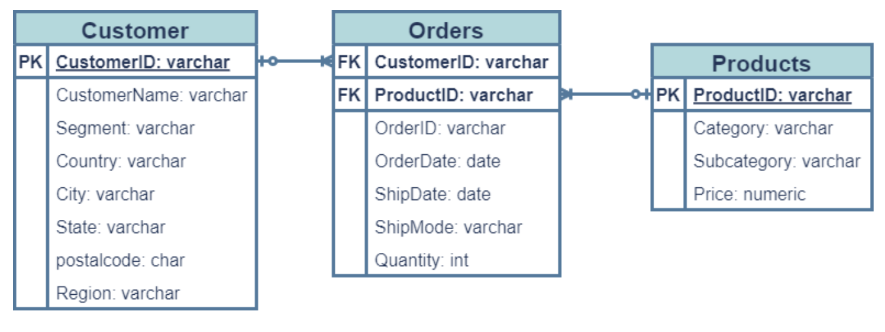
\includegraphics[height=5cm]{resources/2.png}

    Escribe una expresión de álgebra relacional para responder las siguientes consultas. Deberás comprobar cada una ellas
en la calculadora Relax y agregar para cada inciso la expresión en álgebra relacional y una captura de pantalla con el
resultado obtenido (no es necesario mostrar todas las tuplas):
\end{center}
\newpage
